\documentclass[conference]{IEEEtran}
\IEEEoverridecommandlockouts

\usepackage{cite}
\usepackage{amsmath,amssymb,amsfonts}
\usepackage{algorithmic}
\usepackage{graphicx}
\usepackage{textcomp}
\usepackage{xcolor}
\usepackage{float}
\usepackage{tikz}
\usepackage{rotating}
\usepackage[croatian]{babel}


\def\BibTeX{{\rm B\kern-.05em{\sc i\kern-.025em b}\kern-.08em
    T\kern-.1667em\lower.7ex\hbox{E}\kern-.125emX}}
\begin{document}

\title{Generiranje imena naselja pomocu LSTM mreže}


\author{
\IEEEauthorblockN{Antonio Čogelja}
\and
\IEEEauthorblockN{Morena Granić}
\and
\IEEEauthorblockN{Fran Lubina}
\and
\IEEEauthorblockN{Iva Jurković}
\and
\IEEEauthorblockN{Jakov Juvančić}
\and
\IEEEauthorblockN{Matej Logarušić}
}

\maketitle

\begin{abstract}
Cilj projekta je LSTM rekurzivna neuronska mreža na razini znakova koja generira realistična imena hrvatskih naselja. Fokus projekta je treniranje i razvijanje neuronske mreže za generiranje realističnih imena hrvatskih naselja. Korištenjem LSTM mreže, koja je prilagođena za analizu sekvencijskih podataka, cilj je razviti model sposoban za učenje jezičnih obrazaca i struktura iz postojećih imena naselja. Svrha mreže je generiranje novih imena temeljenih na tim naučenim obrascima, pri čemu se zadržavaju jezične i strukturne zakonitosti specifične za taj kontekst.
Željena točnost modela $\eta$ je $\lim_{\tau \to 0} \eta = 0.5$
\end{abstract}

\begin{IEEEkeywords}
Naselje, LSTM, rekurzivne mreže, neuronske mreže-
\end{IEEEkeywords}

\section{Uvod}
\label{sect:intro}
Ishod projekta je LSTM rekurzivna neuronska mreža na razini znakova koja generira realistična imena hrvatskih naselja.\\
Mreža radi sa vektorima koji predstavljaju slova hrvatske abecede proširene specijalnim znakovima $\Sigma = \{ \text{hrv. abeceda}\} \cup \{\langle start \rangle, "\setminus 0"\}$.\\
Ulaz mreže je one-hot vektor $\mathbf{x}^{(t)}$ dimezije $\lvert \Sigma \rvert = 30 + 2$.
\begin{equation}
\mathbf{x}^{(t)}_i=
    \begin{cases}
      1, & \text{ako}\ i=j \\
      0, & \text{inače}
    \end{cases}
\end{equation}
Izlaz dobiven na kraju pojedinog vremenskog koraka $t$ je vektor vjerojatnosti pojave pojednog znaka abecende.\\
\begin{align}
    \hat{\mathbf{y}}^{(t)} &= \begin{bmatrix}
           p(c_0) \\
           p(c_1 | c_0) \\
           \vdots \\
           p(c_{\lvert \Sigma \rvert -1} | \bigcap_{i=0}^{\lvert \Sigma \rvert -2} c_i)
         \end{bmatrix}
         \quad \quad \text{Gdje} \quad c \in \Sigma
\end{align}
Vjerojatnosti su dobivene softmax funkcijom parametriziranom hiperparametrom temperature $\tau$.\\
Na temelju tih vjerojatnosti se uzorkuje konačni izlazni vektor $\mathbf{y}^{(t)}$, odnosno t-ti znak u imenu naselja.\\
\begin{equation}
 \mathbf{y}^{(t)} \sim \hat{\mathbf{y}}^{(t)} = \sigma_{\tau}(f(\mathbf{x}^{(t)} ; \boldsymbol{\theta}))
\end{equation}
\ \\
$f(\mathbf{x} ; \boldsymbol{\theta})$ predstavlja ukupno djelovanje ćelija modela nad njenim ulazom parametrizirano hiperparametrima modela $\boldsymbol{\theta} = \begin{bmatrix} \lvert \mathbf{a} \rvert & \mu & \tau \end{bmatrix}$\\ (opisani u poglavlju \ref{subsect_hiper})
Temperaturno uzorkovanje je izabrano, jer omogućava eksperimentiranje i generiranje zanimljivih toponima.
Izlaz mreže je niz znakova $\{\mathbf{y}^{(t)}\} \biggr \rvert_{t=0}^{T-1}$, odnosno ime naselja.
Željena točnost modela $\eta$ je $\lim_{\tau \to 0} \eta = 0.5$

\section{Pregled literature}
U ovom poglavlju dajemo kratki pregled postojeće literature na način kako je to učinjeno u \cite{Fatima}. Svrstavanjem radova na temelju kriterija: pristupa dubokom učenju, funkciji pogreške, primjeni, jeziku i skupu podataka.\\
Dobivamo taksonomiju na slici \ref{pic:takso}.\\
Nas samo zanimaju radovi na jezicima spomenutim u cjelini \ref{sect:intro} na razini riječi.\\
U konačnici odabiremo karakteristike našeg rješenja, navedene u tablici \ref{tab:karak}.\\


\begin{figure}[H]
\centering
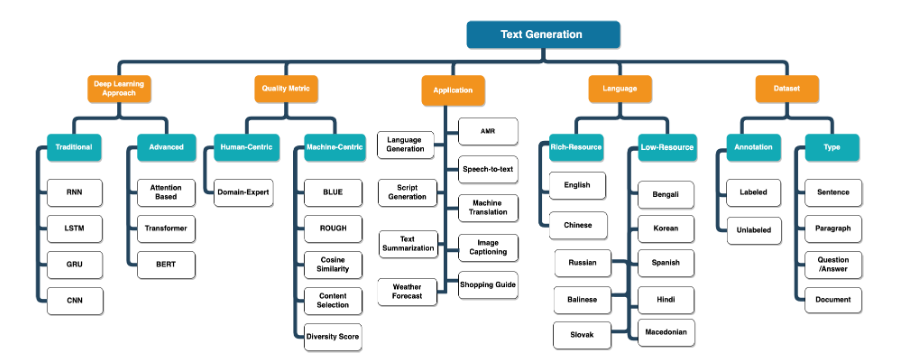
\includegraphics[angle=90, scale=0.3]{./pics/taksonomija.png}\\
\caption{taksonomija rješenja za generiranje teksta}
\label{pic:takso}
\end{figure}

Nas samo zanimaju radovi na jezicima spomenutim u cjelini \ref{sect:intro} na razini riječi sa primjenom generiranja jezičnih konstrukta.\\
U konačnici odabiremo karakteristike našeg rješenja, navedene u tablici \ref{tab:hiper}.\\



\section{Opis implementirane LSTM mreže}
Fokus projekta je treniranje i razvijanje neuronske mreže za generiranje realističnih imena hrvatskih naselja. Korištenjem LSTM mreže, koja je prilagođena za analizu sekvencijskih podataka, cilj je razviti model sposoban za učenje jezičnih obrazaca i struktura iz postojećih imena naselja. Svrha mreže je generiranje novih imena temeljenih na tim naučenim obrascima, pri čemu se zadržavaju jezične i strukturne zakonitosti specifične za taj kontekst.
LSTM ćelija i mreža je implementirana u radnom okviru pyTorch.\\
Dizajn mreže i podešavanje hiperparametara se odvija paralelno sa implementacijom mreže u radnom okviru Keras.

\subsection{Arhitektura}
--

\subsection{Hiperparametri}
\label{subsect_hiper}

\begin{table}[htbp]
\caption{hiperparametri naše mreže}
\begin{center}
\begin{tabular}{|c|c|c|}
\hline
\textbf{Hiperparametar} & \textbf{\textit{Vrijednost}} & \textbf{\textit{komentar}}\\ \hline
broj jedinica po sloju & 2 & \\ \hline
stopa učenja ($\mu$) &  & \\ \hline
temperatura ($\tau$) &  & \\ \hline
dimenzija skrivenog stanja ($\lvert \mathbf{a} \rvert$) &  & \\ \hline
broj epoha & 100 & \\ \hline \hline
aktivacijska funckija & tanh & zadano \\ \hline
povratna akt. funkcija & $\sigma_{\tau}$ & zadano \\ \hline
bias & da & zadano \\ \hline
inicijalizator kernela & glorot jednoliki & zadano \\ \hline
inicijalizator povratne veze & glorot jednoliki & zadano \\ \hline
bias inicijalizator & zeros & zadano \\ \hline
forget bias & da & zadano \\ \hline
regularizacija kernela & & zadano \\ \hline
regularizacija kernela povratne veze &  & zadano \\ \hline
bias regularizacija &  & zadano \\ \hline
kernel ograničenje &  & zadano \\ \hline
povratno ograničenje &  & zadano \\ \hline
bias ograničenje & & zadano\\ \hline
dropout & 0 & zadano \\ \hline
povratni dropout & 0 & zadano \\ \hline
\end{tabular}
\label{tab:hiper}
\end{center}
\end{table}



\subsection{Ćelija}
Ćelija izgledda ovako.

\begin{figure}
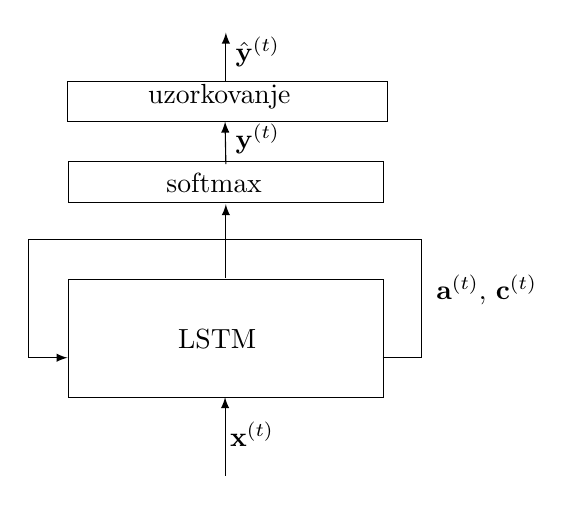
\begin{tikzpicture}
	\draw[draw=black, thin, solid] (-2.99,5.49) rectangle (1.01,4.00);
	\node[black, anchor=south west] at (-1.72,4.49) {LSTM};
	\draw[draw=black, -latex, thin, solid] (-1.00,3.00) -- (-1.00,4.00);
	\draw[draw=black, -latex, thin, solid] (-0.99,5.51) -- (-0.99,6.45);
	\draw[draw=black, thin, solid] (1.00,4.50) -- (1.50,4.50);
	\draw[draw=black, thin, solid] (1.50,4.50) -- (1.50,6.00);
	\draw[draw=black, thin, solid] (1.50,6.00) -- (-3.50,6.00);
	\draw[draw=black, thin, solid] (-3.50,6.00) -- (-3.50,4.50);
	\draw[draw=black, -latex, thin, solid] (-3.50,4.50) -- (-3.00,4.50);
	\draw[draw=black, thin, solid] (-2.99,6.99) rectangle (1.01,6.47);
	\node[black, anchor=south west] at (-1.87,6.47) {softmax};
	\node[black, anchor=south west] at (-0.99,6.96) {$\mathbf{y}^{(t)}$};
	\node[black, anchor=south west] at (-1.06,3.25) {$\mathbf{x}^{(t)}$};
%	\node[black, anchor=south west] at (-1.09,5.92) {$f(\mathbf{x}^{(t)})$};
	\draw[draw=black, -latex, thin, solid] (-0.99,6.96) -- (-1.00,7.50);
	\draw[draw=black, thin, solid] (-3.00,7.50) rectangle (1.06,8.01);
	\node[black, anchor=south west] at (-2.10,7.54) {uzorkovanje};
	\node[black, anchor=south west] at (-0.99,8.07) {$\hat{\mathbf{y}}^{(t)}$};
	\draw[draw=black, -latex, thin, solid] (-0.99,8.02) -- (-0.99,8.63);
	\node[black, anchor=south west] at (1.56,5.05) {$\mathbf{a}^{(t)}$, $\mathbf{c}^{(t)}$};
\end{tikzpicture}
\caption{Arhitektura LSTM ćelije}
\end{figure}
\ \\
Nadalje slika \ref{tikz:detail} prikazuje unutarnju shemu ćelije.

\begin{sidewaysfigure*}
\resizebox{550pt}{!}{
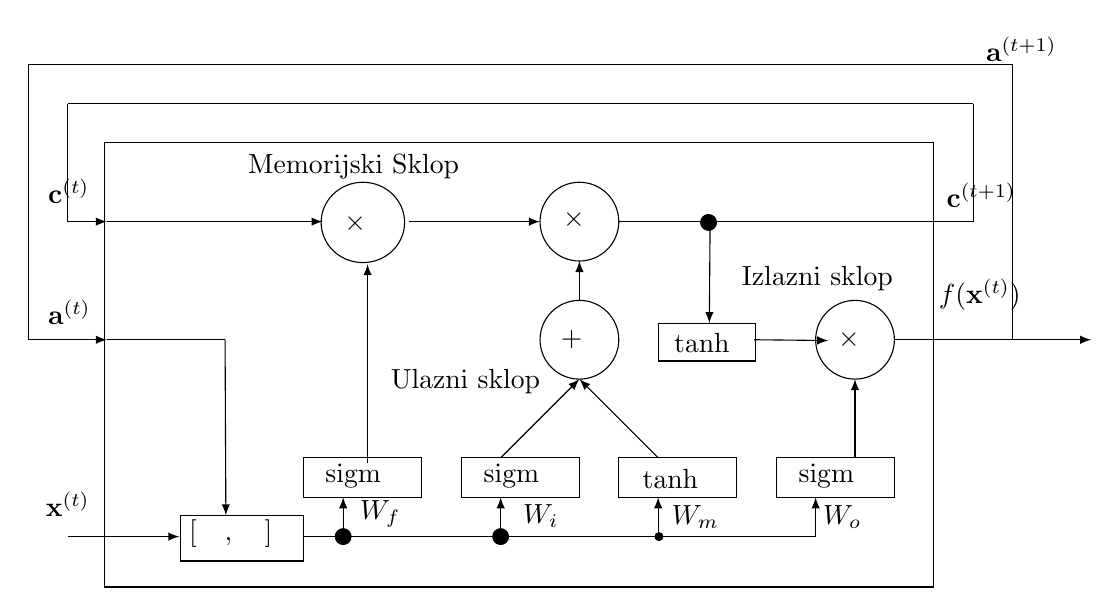
\begin{tikzpicture}
\label{tikz:detail}
	\draw[draw=black, thin, solid] (-5.03,0.86) rectangle (5.50,6.50);
	\draw[draw=black, thin, solid] (4.50,4.00) ellipse (0.50 and -0.50);
	\draw[draw=black, thin, solid] (1.00,4.00) ellipse (0.50 and -0.50);
	\draw[draw=black, thin, solid] (1.00,5.50) ellipse (0.50 and -0.50);
	\draw[draw=black, thin, solid] (-1.75,5.49) ellipse (0.53 and 0.51);
	\draw[draw=black, thin, solid] (1.50,2.00) rectangle (3.00,2.50);
	\draw[draw=black, thin, solid] (-0.50,2.50) rectangle (1.00,2.00);
	\draw[draw=black, thin, solid] (-2.50,2.00) rectangle (-1.00,2.50);
	\draw[draw=black, thin, solid] (-4.07,1.77) rectangle (-2.50,1.19);
	\draw[draw=black, thin, solid] (3.50,2.00) rectangle (5.00,2.50);
	\node[black, anchor=south west] at (2.08,3.72) {tanh};
	\node[black, anchor=south west] at (1.68,1.99) {tanh};
	\node[black, anchor=south west] at (-2.35,2.00) {sigm};
	\node[black, anchor=south west] at (3.66,1.99) {sigm};
	\node[black, anchor=south west] at (-0.34,1.99) {sigm};
	\node[black, anchor=south west] at (-4.08,1.24) {$[\quad , \quad]$};
	\node[black, anchor=south west] at (-1.52,3.19) {Ulazni sklop};
	\node[black, anchor=south west] at (2.94,4.50) {Izlazni sklop};
	\node[black, anchor=south west] at (-3.33,5.92) {Memorijski Sklop};
	\node[black, anchor=south west] at (-1.91,1.49) {$W_f$};
	\node[black, anchor=south west] at (0.16,1.49) {$W_i$};
	\node[black, anchor=south west] at (2.05,1.48) {$W_m$};
	\node[black, anchor=south west] at (3.97,1.48) {$W_o$};
	\node[black, anchor=south west] at (-5.87,4.07) {$\mathbf{a}^{(t)}$};
	\node[black, anchor=south west] at (6.04,7.41) {$\mathbf{a}^{(t+1)}$};
	\node[black, anchor=south west] at (5.54,5.55) {$\mathbf{c}^{(t+1)}$};
	\node[black, anchor=south west] at (-5.87,5.60) {$\mathbf{c}^{(t)}$};
	\node[black, anchor=south west] at (5.44,4.25) {$f(\mathbf{x}^{(t)})$};
	\node[black, anchor=south west] at (-5.90,1.63) {$\mathbf{x}^{(t)}$};
	\node[black, anchor=south west] at (-2.11,5.23) {$\times$};
	\node[black, anchor=south west] at (0.67,5.28) {$\times$};
	\node[black, anchor=south west] at (4.16,3.76) {$\times$};
	\node[black, anchor=south west] at (0.64,3.76) {$+$};
	\draw[draw=black, thin, solid] (2.00,3.73) rectangle (3.24,4.21);
	\draw[draw=black, -latex, thin, solid] (-1.69,2.44) -- (-1.69,4.96);
	\draw[draw=black, -latex, thin, solid] (-5.00,5.50) -- (-2.26,5.50);
	\draw[draw=black, -latex, thin, solid] (-1.17,5.50) -- (0.50,5.50);
	\draw[draw=black, -latex, thin, solid] (1.00,4.50) -- (1.00,5.00);
	\draw[draw=black, -latex, thin, solid] (0.00,2.50) -- (1.00,3.50);
	\draw[draw=black, -latex, thin, solid] (2.00,2.50) -- (1.00,3.50);
	\draw[draw=black, -latex, thin, solid] (-0.00,1.51) -- (0.00,2.00);
	\draw[draw=black, -latex, thin, solid] (2.00,1.50) -- (2.00,2.00);
	\draw[draw=black, -latex, thin, solid] (4.00,1.50) -- (4.00,2.00);
	\draw[draw=black, -latex, thin, solid] (-2.00,1.50) -- (-2.00,2.00);
	\draw[draw=black, thin, solid] (-2.50,1.50) -- (4.00,1.50);
	\draw[draw=black, fill=black, thin, solid] (2.01,1.50) ellipse (0.05 and -0.05);
	\draw[draw=black, -latex, thin, solid] (-5.50,1.50) -- (-4.08,1.50);
	\draw[draw=black, -latex, thin, solid] (3.22,4.00) -- (4.16,3.99);
	\draw[draw=black, -latex, thin, solid] (-5.50,5.50) -- (-5.00,5.50);
	\draw[draw=black, -latex, thin, solid] (-3.50,4.00) -- (-3.49,1.77);
	\draw[draw=black, -latex, thin, solid] (4.50,2.50) -- (4.50,3.50);
	\draw[draw=black, -latex, thin, solid] (2.66,5.51) -- (2.65,4.21);
	\draw[draw=black, fill=black, thin, solid] (-2.00,1.50) circle (0.1);
	\draw[draw=black, fill=black, thin, solid] (0.00,1.50) circle (0.1);
	\draw[draw=black, fill=black, thin, solid] (2.64,5.49) circle (0.1);
	\draw[draw=black, thin, solid] (5.00,4.00) -- (6.50,4.00);
	\draw[draw=black, thin, solid] (6.50,4.00) -- (6.50,7.50);
	\draw[draw=black, thin, solid] (6.50,7.50) -- (-6.00,7.50);
	\draw[draw=black, thin, solid] (-6.00,7.50) -- (-6.00,4.00);
	\draw[draw=black, -latex, thin, solid] (-6.00,4.00) -- (-5.00,4.00);
	\draw[draw=black, thin, solid] (-5.00,4.00) -- (-3.50,4.00);
	\draw[draw=black, -latex, thin, solid] (6.50,4.00) -- (7.50,4.00);
	\draw[draw=black, thin, solid] (1.50,5.50) -- (6.00,5.50);
	\draw[draw=black, thin, solid] (6.00,5.50) -- (6.00,7.00);
	\draw[draw=black, thin, solid] (6.00,7.00) -- (-5.50,7.00);
	\draw[draw=black, thin, solid] (-5.50,7.00) -- (-5.50,5.50);
\end{tikzpicture}
}
\caption{Unutarnja arhitektura LSTM ćelije}
\end{sidewaysfigure*}

\subsection{Treniranje}
BPTT je korišten kao algoritam učenja.
Kao funkcija gubitka koristi se unakrsna entropija.
\begin{equation}
L_i = - \sum_{t = 0}^{T-1} \mathbf{x}_i^{(t)} \cdot log(\hat{\mathbf{y}}_i^{(t)})
\end{equation}
inačica BPTT koju mi koristimo je u biti propagirani stohastički gradijentni spust.\\
\\
Pri treniranju koristimo parametre navedene u tablici \ref{tab:trening}.
\begin{table}[htbp]
\caption{parametri procedure za treniranje}
\begin{center}
\begin{tabular}{|c|c|}
\hline
\textbf{Parametar} & \textbf{\textit{Vrijednost}}\\ \hline
f-ja gubitka & kategorička unakrsna entropija \\ \hline
algoritam optimizacije & ADAM \\ \hline
metrike & točnost \\ \hline
\end{tabular}
\label{tab:trening}
\end{center}
\end{table}

\section{Opis eksperimentalnih rezultata}\label{FAT}
\paragraph{optimiranje hiperparametara}
--

\begin{table}[htbp]
\caption{Table Type Styles}
\begin{center}
\begin{tabular}{|c|c|c|c|}
\hline
\textbf{Table}&\multicolumn{3}{|c|}{\textbf{Table Column Head}} \\
\cline{2-4} 
\textbf{Head} & \textbf{\textit{Table column subhead}}& \textbf{\textit{Subhead}}& \textbf{\textit{Subhead}} \\
\hline
copy& More table copy$^{\mathrm{a}}$& &  \\
\hline
\multicolumn{4}{l}{$^{\mathrm{a}}$Sample of a Table footnote.}
\end{tabular}
\label{tab1}
\end{center}
\end{table}

\subsection{Usporedba rezultata}
--

\section{Zaključak}
--


\begin{thebibliography}{00}
\bibitem{Fatima} Fatima, N., Imran, A S., Kastrati, Z., Daudpota, S M., Soomro, A (2022) ``A Systematic Literature Review on Text Generation Using Deep Neural Network Models``
IEEE Access, 10: 53490-53503, https://doi.org/10.1109/ACCESS.2022.3174108
\end{thebibliography}



\end{document}
